\section{Background on graphics processing units (GPUs)}

\begin{frame}[t]
\frametitle{Introduction}
\begin{columns}[T]
\begin{column}{0.5\textwidth}
\begin{itemize}
\item Highly multi-threaded processor
    \begin{itemize}
        \item NVIDIA Tesla K20 accelerator: 2496 cores
    \end{itemize}
\item Spectacular performance for
    \emph{compute-intensive, data-parallel} operations
\item Not suited for general-purpose computation
\item Requires careful redesign of algorithms,
    substantial code changes, and tuning efforts
\end{itemize}
\end{column}
\begin{column}{0.5\textwidth}
\begin{figure}
\begin{center}
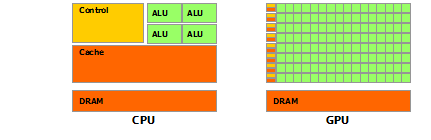
\includegraphics[width=150px]{img/device-comparison.png}
\centering
\caption{Design philosophy of GPU (CUDA Programming Guide)}
\end{center}
\end{figure}
\end{column}
\end{columns}
\end{frame}

\begin{frame}
\frametitle{CUDA Programming model}
\begin{itemize}
\item Several options for programming GPUs
    \begin{itemize}[<+->]
        \item underlying models: CUDA and OpenCL
    \end{itemize}
\item Important to understand for good performance
\item Primary features:
    \begin{itemize}
        \item \emph{Kernels} and thread organization
        \item GPU Architecture
        \item Memory hierarchy
    \end{itemize}
\end{itemize}
\end{frame}

\begin{frame}
\frametitle{Kernels and thread organization}
\begin{columns}
\begin{column}{0.5\textwidth}
\textbf{Kernels}
\begin{itemize}
\item Special pieces of code that execute on the GPU
\item In Fortran: subroutines; in C: functions
\item Executed concurrently by several GPU threads
\end{itemize}
\textbf{Threads}
\begin{itemize}
\item Threads organized into a grid of blocks
\item Kernels launched with specified grid size
    (number of blocks) and block size (threads per block)
\item Grid and blocks can be 2-D or 3-D for convenience
\end{itemize}
\end{column}
\begin{column}{0.5\textwidth}
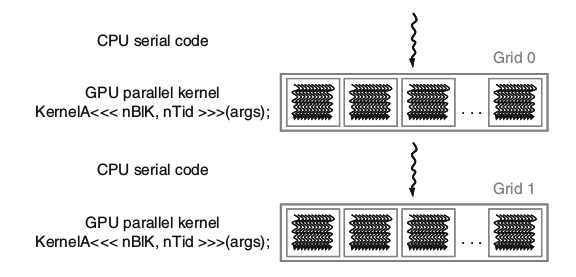
\includegraphics[width=120px]{img/program-structure.png}
\vspace{1cm}
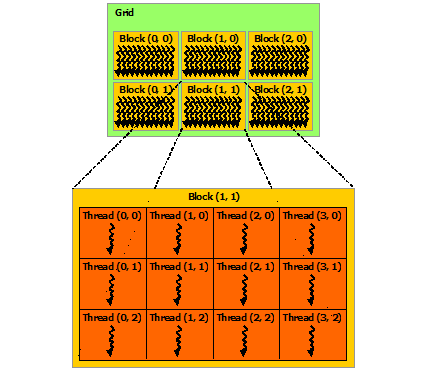
\includegraphics[width=120px]{img/grid-of-thread-blocks.png}
\end{column}
\end{columns}
\end{frame}

\begin{frame}
\frametitle{GPU Architecture}
\begin{columns}
\begin{column}{0.5\textwidth}
\begin{itemize}
\item GPU viewed as a collection of \emph{streaming microprocessors} (SMs)
\item When kernel is launched, each block gets assigned to an SM
\item Threads within a block execute concurrently
\item SM may execute several blocks concurrently
\end{itemize}
\end{column}
\begin{column}{0.5\textwidth}
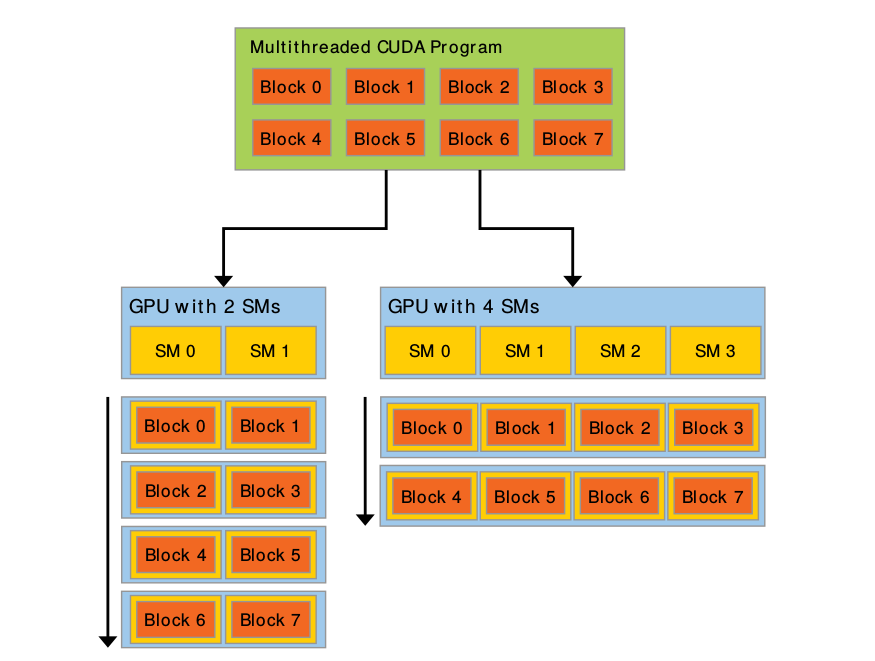
\includegraphics[width=150px]{img/gpu-scaling.png}
\end{column}
\end{columns}
\end{frame}

\begin{frame}
\frametitle{Memory hierarchy}
\begin{columns}
\begin{column}{0.5\textwidth}
\begin{itemize}
\item Global memory{
\begin{itemize}
    \item large but slow (~5 GB for Tesla K20)
    \item CPU can access (via PCI-e bus)
    \item all threads can access
    \item persists between kernel launches
\end{itemize}}
\item Shared memory{
\begin{itemize}
    \item small but fast (~48 KiB per SM and block)
    \item local to threads within a block
    \item threads in a block read and write into shared memory
    \item explicitly managed cache
\end{itemize}}
\item Registers{
\begin{itemize}
    \item limited (65536 per SM and block)
    \item local to individual threads
    \item fastest
\end{itemize}}
\end{itemize}
\end{column}
\begin{column}{0.5\textwidth}
    \visible{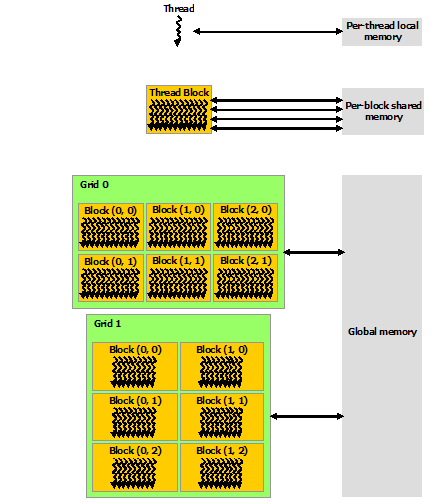
\includegraphics[width=150px]{img/memory-hierarchy.png}}
\end{column}
\end{columns}
\end{frame}

\begin{frame}
\frametitle{Performance considerations}
\begin{itemize}
\item CPU-GPU transfers
\item Coalesced global memory access
    \begin{itemize}
        \item successive threads must access nearby locations
    \end{itemize}
\item Shared memory and bank conflicts
    \begin{itemize}
        \item \emph{strided} memory access is serialized
    \end{itemize}
\item Limiting use of shared memory and registers
\end{itemize}
\end{frame}

